\section{本章小结}

本章介绍了指数函数和对数函数。
关键点:
\begin{itemize}
    \item 指数函数和对数函数可通过等比数列加深理解;
    \item 两者是互为反函数;
    \item 熟悉使用指数函数和对数函数作为模型求解实际问题。
\end{itemize}

~

\begin{example}[复习巩固4,难度:$\star $]
已知函数
\[
f\left( x \right) =\begin{cases}
	x^2+2x-3 &x\leqslant 0\\
	-2+\ln x &x>0\\
\end{cases}
\]
求使方程$f\left( x \right) =k$的实数解个数分别为1、2、3时$k$的相应取值范围。
\end{example}

解:

首先观察
\[
-2+\ln x-k=0 \qquad x>0
\]
即函数$g\left( x \right) =\ln x-\left( k+2 \right) $,相比$\ln x$往下移了$k+2$,无论如何都跟{\it x}轴有且仅有一个交点。所以本题实际为考察
\[
g\left( x \right) =x^2+2x-3-k \qquad x\leqslant 0
\]
与{\it x}轴的交点。
方程化为:
\[
g\left( x \right) =\left( x+1 \right) ^2+\left( -4-k \right)
\]
即将$\left( x+1 \right) ^2$上下平移得到,易得:
\begin{itemize}
    \item $-4-k>0$时,无交点;
    \item $-4-k=0$或$-4-k<-1$时,1个交点;
    \item 其余,2个交点。
\end{itemize}

\begin{tcolorbox}
本题没啥难度,考察幂函数和对数函数的形态而已。
\end{tcolorbox}

~

\begin{example}[拓广探索12,难度:$\star $]
对于函数
\[
f\left( x \right) =a-\frac{2}{2^x+1} \qquad a\in \mathbb{R}
\]
\begin{enumerate}
    \item 探索函数$f\left( x \right) $的单调性;
    \item 是否存在实数$a$使函数$f\left( x \right) $为奇函数?
    \item (附加)证明函数是中心对称。
\end{enumerate}
\end{example}

解:

(1)从定义出发,令$x_1<x_2$,则有:
\begin{align*}
f\left( x_1 \right) -f\left( x_2 \right) &=\frac{2}{2^{x_2}+1}-\frac{2}{2^{x_1}+1}=2\cdot \frac{\left( 2^{x_1}+1 \right) -\left( 2^{x_2}+1 \right)}{\left( 2^{x_2}+1 \right) \left( 2^{x_1}+1 \right)} \\
&=2\cdot \frac{2^{x_1}-2^{x_2}}{\left( 2^{x_2}+1 \right) \left( 2^{x_1}+1 \right)}<0
\end{align*}

(2)若要使$f\left( x \right) $为奇函数,则必须$f\left( -x \right) =-f\left( x \right) $,于是:
\begin{align*}
&\because f\left( -x \right) =a-\frac{2}{2^{-x}+1}=a-\frac{2}{\frac{1}{2^x}+1}=\frac{a\left( 2^x+1 \right) -2\cdot 2^x}{2^x+1} \\
&\because -f\left( x \right) =\frac{-a\left( 2^x+1 \right) +2}{2^x+1} \\
&\therefore \left( a-2 \right) \cdot 2^x+a=-a\cdot 2^x-a+2 \\
&\therefore \left( a-1 \right) \cdot 2^x=-\left( a-1 \right)
\end{align*}
可见,$a=1$即可,带入验证:
\begin{align*}
&f\left( x \right) =1-\frac{2}{2^x+1}=\frac{2^x-1}{2^x+1} \\
&f\left( -x \right) =\frac{2^{-x}-1}{2^{-x}+1}=\frac{\frac{1}{2^x}-\frac{2^x}{2^x}}{\frac{1}{2^x}+\frac{2^x}{2^x}}=\frac{1-2^x}{1+2^x}
\end{align*}

\begin{figure}[h]
\centering
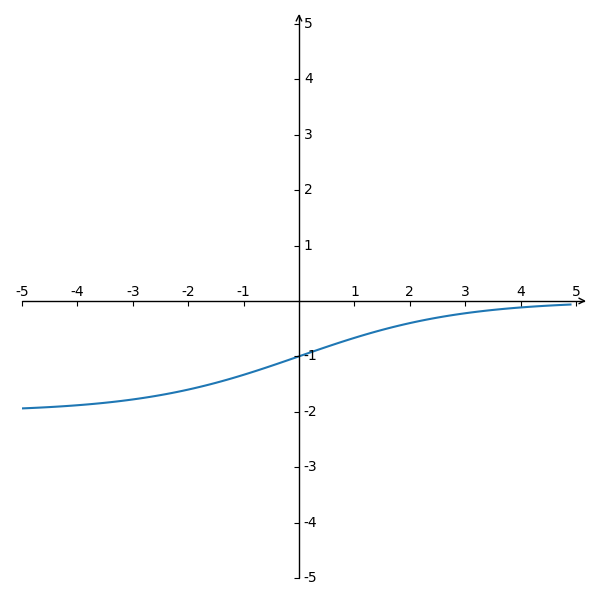
\includegraphics[height=6cm]{4.6-1.png}
\end{figure}

(3)中心对称即若有$x_1+x_2=2x_0$则有$y_1+y_2=2y_0$,带入计算:
\begin{align*}
y_1+y_2&=a-\frac{2}{2^{x_1}+1}+a-\frac{2}{2^{x_2}+1} \\
&=2a-2\cdot \frac{2^{x_1}+2^{x_2}+2}{2^{x_1+x_2}+2^{x_1}+2^{x_2}+1}
\end{align*}
可见,当$x_1+x_2=0$时,有$y_1+y_2=2a-2$,也即中心点$\left( 0,2a-2 \right) $。

回头再看(2),只需要上抬就可以满足奇函数要求。

\begin{tcolorbox}
本题从定义出发即可。
本题的附加(3)类似2024年高考第18题。
\end{tcolorbox}




